\documentclass[a4paper]{article}
\usepackage[utf8]{inputenc}
\usepackage[Slovene]{babel}
\usepackage{graphicx}
\usepackage{tikz}
\usepackage{pdfpages}

\usepackage{nameref}

\usepackage{amsmath}
\usepackage{amsfonts}
\usepackage{amssymb}
\usepackage{makeidx}
\usepackage{graphicx}
\usepackage{fourier}

\usepackage{circuitikz}
\usetikzlibrary{circuits.logic.IEC}

\usepackage{fancyhdr}
\pagestyle{fancy}
\lhead{Mitja Alič}
\rhead{DIGITALNI MERILNIK VRTILNE HITROSTI }
\cfoot{\thepage}



% mapa s slikami
\graphicspath{{./Slike/}}


\begin{document}


\begin{titlepage}
	\centering

	{\scshape\LARGE Univerza v Ljubljani \par}
	{\scshape\large Fakulteta za elektrotehniko \par}
	\vspace{3cm}
	{\scshape\Large Poro\v cilo pri predmetu seminar iz mehatronike\par}
	\vspace{1.5cm}
	{\huge\bfseries DIGITALNI MERILNIK VRTILNE HITROSTI\par}
	\vspace{2cm}
	{\Large Mitja Ali"c\par}
	\vspace{0.5cm}
	Profesor:\par
	prof.~dr.~Danijel Von"cina\par
		\vspace{0.25cm}
	Mentor:\par
	doc.~dr.~Mitja Nemec\par
	

	\vfill

% Bottom of the page
	{\large Ljubljana, 2017\par}
\end{titlepage}


\tableofcontents

\newpage

\section{Uvod}
Pri predmetu seminar iz mehatronike sem si izbral projekt izdelave digitalneg merilnika vrtilne hitrosti. Pri delu na projektu, bom osvojil znanje risanje sheme o"zi"cenja, risanja tiskanega vezja, izdelava vezja in testiranje. V povezavi s predmetom digitalno procesiranje v mehatroniki 2 (v nadaljevanju DP2), bom napisal program za dolo"canje vrtilne hitrosti na podlagi poznavanja tenutnega kota zasuka. Cilj izdelanega vezja, je analogni prikaz vrtilne hitrosti na izhodu, katero bi lahko "studentje opazovali na laboratorijskih vajah. Podobno seminarsko nalogo je imel "Ziga Prajndl\footnote{Digitalni merilnik hitrosti, "Ziga Prajndl, LRTME, Ljubljana, 2016} leto prej, kjer je uporabil F28069 Piccolo controlSTICK. Piccolo se uporablja pri laboratorijskih vajah predmeta DP2. Na tem "cipu naj izdelal salgoritem, nato pa ga prenesel na svojo tiskanino, kjer bi uporabil drug mikrokrmilnik.

\section{Zahteve}

Na za"cetku sem si prebral poro"cilo mojega predhodnika in njegove zahteve prilagodil. Osnovne zahteve so bile enake. Blokovna shema je na sliki \ref{fig:blokovna}.  Tiskanina bo priklju"cena na 5 V napajalni vir. Ostale napetosti so generirane s DC-DC pretvornikom. Za znane komponente sem pregledal podatkovne liste in za"cel graditi shemo.

\begin{figure}[h!]
	\centering
	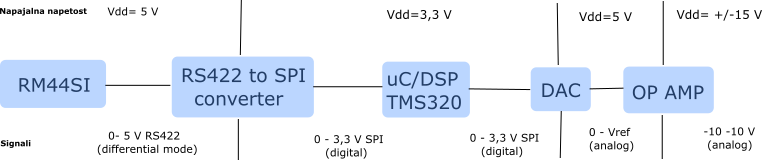
\includegraphics[width=\linewidth]{blokovna_shema.png}
	\caption{Blokovna shema merilnika z vrednostmi napajalnih napetosti in velikkostjo napetostnih siganlov}
	\label{fig:blokovna}
\end{figure}

Za prera"cunavanje in komunikacijo sem uporabil mikro krmilni TMS320F28027. Izvorno informacijo o kotu zasuka gredi elektromotorskega sklopa prejemamo iz absolutnega dajalnika zzasuka podjetja RLS z oznako RM44SI0012B30F2E10. Izhod senzorja je lahko inkremantalni z referen"cno to"cko, v obliki analognih potekov sinusa in kosinusa, ali preko serijske komunikacije. Komunikacija deluje v diferencialnem na"cinu, kar pove"ca zanesljivost prenosa. Mikrokrmilnik podpira komunikacijo SPI, zato je potrebno uporabiti gonilik ki pretvori diferencialna signala v  polariziran signal. Uporabil sem integrirano vezje SN65HVD73.

Na izhodni strani aplikacije "zelimo podatek o poziciji in posledi"cno hitrosti na"sega pogona po"siljati naprej v analogni obliki za nadaljno regulacijo. Potrebna sta dva analogna izhoda zato sem uporabil TLV5618A. Gre za dvokanalni 12-bitni digitalno analogni pretvornik (DAC). Za vi"sino referen"cne napetosti Vref sem izbral napetost 4,096~V. Napetost sem generiral s LM4132BMF-4.1. 

Tako komunikacija s senzorjem kot tudi z DAC-om zahteva SPI povezavo. Mikrokrmilnik ima le eno SPI enoto. Predhodnik je ugotovil, da lahko senzor in DAC poganja le z eno SPI enoto. Master-input slave-output (MISO) signal slu"zi za prejemanje podatkov s senzorja. Master-output slave-input (MOSI) signal po"slje podatke na DAC. Uro komunikacijskega modula je povezana na obe enoti. 

Za zagotovitev "zeljenih izhodnih napetosti izhoda DAC-a oja"cam s operacijskim oja"cevalnikom. Zahteva mentorja je bila , da ima operacijski oja"cevalnik "cim manj"so sofazno oja"cenje ter naj se vsi nahajajo v enem ohi"sju. Uporabil sem oja"cevaljnik OPA4192IPW. Potreboval sem bipolarno napajanje +/- 15~V, ki sem ga generiral s pretvornikom TMH515D.

Prisotnost napajanja prikazujem na rumeni LED diodi, priklju"ceni na osnovno napajalno napetost 5~V. Z zeleno LED diodo sem prikazoval trenutno vrednost senzorja. S spreminjanjem pozicija se je spreminjala svetilnost LED diode. To sem izvedel s PWM enoto in tranzistorjem serijsko vezanega s LED diodo. Svetilnost LED diode je tako odvisna od preklopnega razmerja PWM enote. Enako sem storil za rde"co led diodo,ki je predstavljala absolutno vrednost hitrosti.


%Moja naloga je sestaviti vezje napajano s 5~V, na katero se priklopi senzor zasuka RM44SI. Izhoda vezja sta analogna signala kota zasuka in hitrosti v razponu med -10~V in 10~V. Enake zahteve je imel "ze moj predhodnik, le da je na tiskanino priklopi Piccolo controlstick, jaz pa sem na tiskanino dal mikrokontroler.
%
%\section{Dolo"canje elementov}
%
%V novembru 2016 sem se lotil izdelave sheme in hkrati dolo"canja elementov. Okvirno shemo mi je sestavil "ze Prajndl. Shemi sem moral dodati "se mikrokrmilnik in kar spada k temu (napajalnik zanj, JTAG konektor).
%
%\subsection{Mikrokrmilnik}
%Mentor mi je predalgal naj vzamem krmilnik iz serije C2000 podjetja Texas Instruments, kateri podira SPI komunikacijo, je "cim manj"si in je dobavljiv na Farnell-u. Odlo"cil sem se za krmilnik TMS320F28027. Ima samo en SPI modul katerega sem uporabil tako, da sem pin za po"siljanje vezal na digitalno analogni pretvornik (v nadeljevanju DAC), pin za sprejemanje pa povezal s senzorjem.
%
%\subsection{Komunikacijski pretvornik}
%
%Senzor zasuka podjetja RLS, RM44SI deluje po komunikaciji RS422, zato sem uporabil vmesnik SN65HVD73 za pretvorbo komunikacije.
%
%\subsection{Tranzistorji za PWM}
%
%Za krmiljeneje LED diod s PWM enoto sem izbral tranzistorje 2N7002KT1G podjetja Semiconductor. Je v ohi"sju SOT23 katero enako ohi"sje imajo tudi tranzistorji uporabljeni pri projektu Prajndla(BSS138). Ker so tranzistorji BSS138 "ze v laboraratoriju sem uporabil te in ni bilo potrebno naro"cilo drugih. 
%
%
%\subsection{Digitalno analogni pretvornik}
%
%Prajndl je uporabil na svojem vezju DAC TLV5610 z osmimi izhodi katerega je opisal prof. Ambro"zi"c na predavanjih DP2. Na izhodu sem potreboval le dva kanala (kot in vrtinlna hitrost), zato sem uporabil DAC TLV5618A z dvema izhodoma.
%
%
%\subsection{Operacijski oja"cevalnik}
%
%"Zelja mentorja je bila uporabiti operacijski oja"cevalnik s "cim manj"so offset napetostjo in vsemi oja"cevalniki v enem ohi"sju. Na podlagi zahtev sem izbral OPA4192ID. Izhod oja"cevalnika mora biti med -10~V in +10~V zato sem napajanje oja"cevalnika dobil z DC-DC pretvornika TMA 0515D podjetja Traco Power.  

\section{Sestava sheme}
\label{shema}
Shemo sem delal v programu Altium Designer 16.1. Celotna shema se nahaja v \nameref{Dodatek1}.




Mentor mi je poslal svoje starej"se projekte, po katerih sem nato povezal pine mikrokrmilnika (Slika \ref{fig:uCshema}). Ob njemu je postavljen JTAG konektor. GPIO in PWM pine sem po mikrokrmilniku razporedil tako, da so mi na tiskanini "cim bolje ustrezali.
	\begin{figure}[h!]
		\centering
		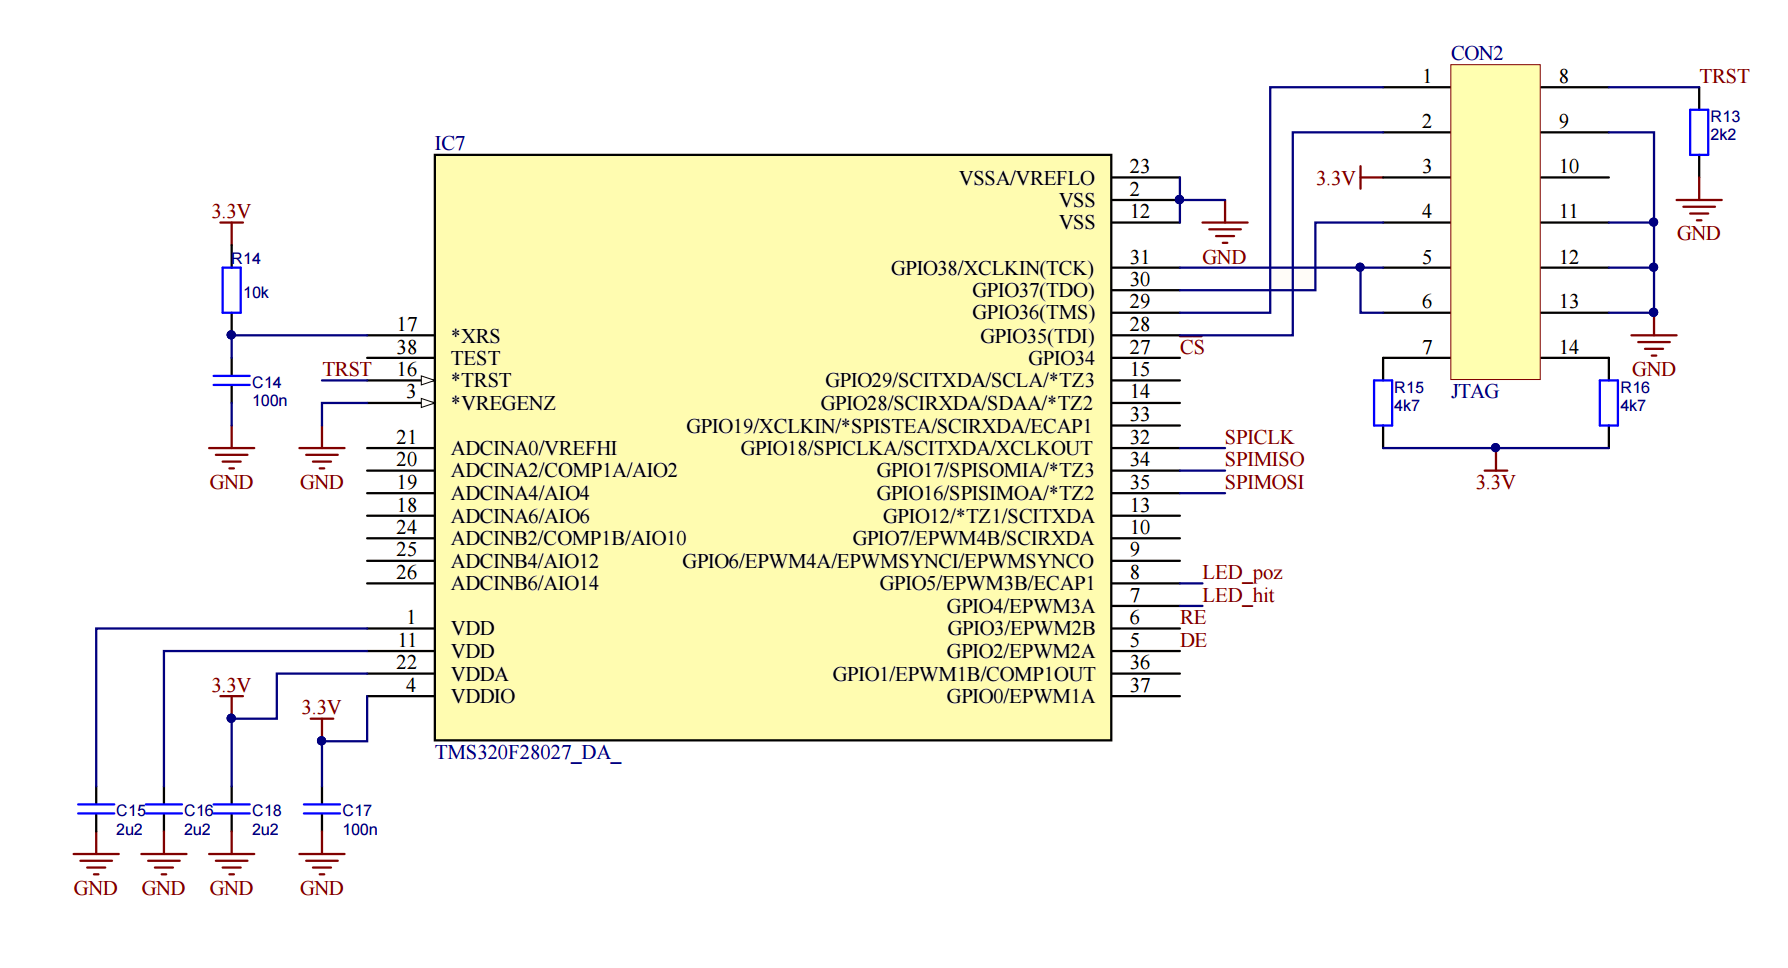
\includegraphics[width=\textwidth]{uC.png}
		\caption{Shema mikrokrmilnika}
		\label{fig:uCshema}
	\end{figure}


PWM pina sem povezal s tranzistorjema (Slika~\ref{fig:LEDshema}), kjer nisem povezal upora na maso ("pull-down"). Tako je na gate-u MOS-FET-a lahko ob nepri"cakovanem dogodku (nedefiniran izhod PWM enote) ostal naboj in posledi"cno je LED dioda svetila.

	\begin{figure}[h!]
		\centering
		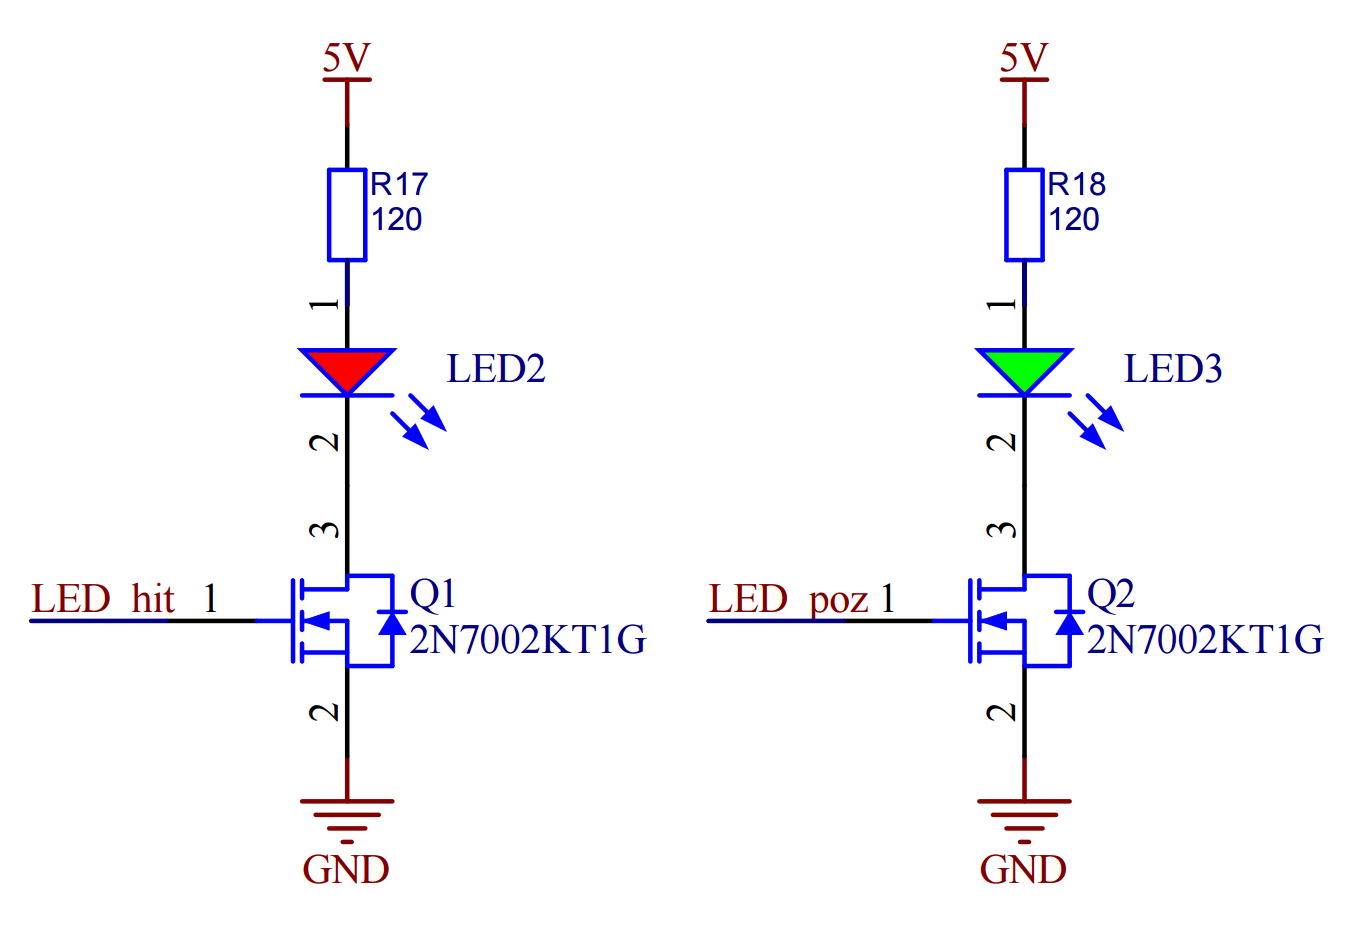
\includegraphics[width=0.5\textwidth ]{LED.png}
		\caption{Shema krmiljenja LED diod}
		 \label{fig:LEDshema}
	\end{figure}
Pri povezavi pretvornika komunikacije je predhodnik naredil lapsus (zamenjal para ure in podatka na SN65HVD73). To sem zamenjal, nisem pa zamenjal tudi elemntov. Med izhodom senzorja zasuka mora biti paralelno vezan 120 $\mathrm{\Omega}$ upor in manj"si kondenzator. To pa sem obdr"zal med povezavama +CLK~-CLK. Tekom projekta sem ugotovil, da je to napaka. Upor R10 in kondenzator C12 (Slika \ref{SPIshema}), bi se morala nahajati med +DAT in -DAT. Upora R11 in R12 bi morala biti na povezavi +CLK oz -~CLK.

	\begin{figure}[h!]
		\centering
		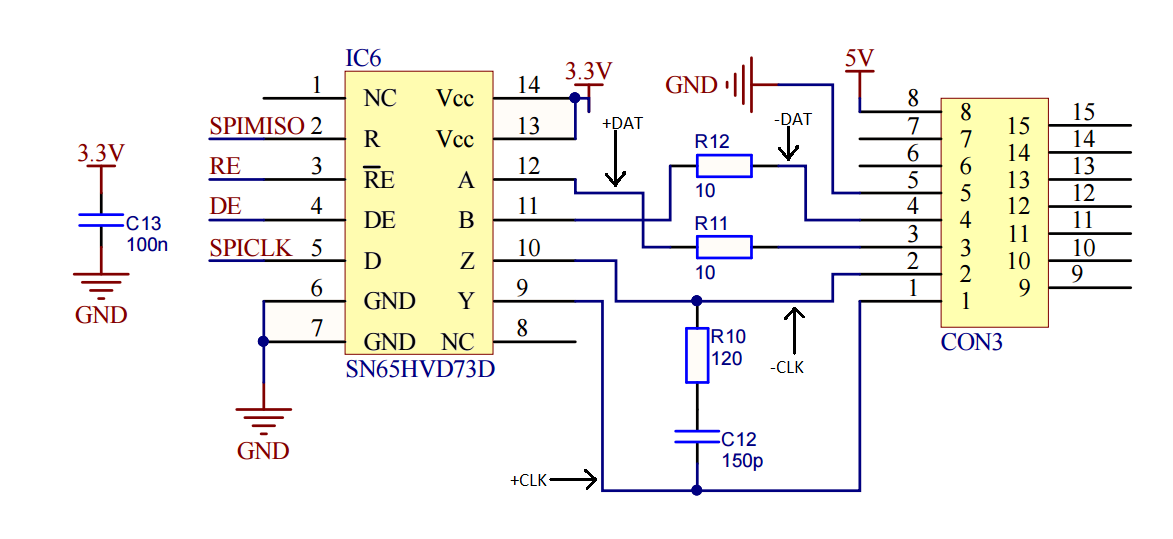
\includegraphics[width=\textwidth]{SPI_interface.png}
		\caption{Shema komunikacije s senzorjem zasuka}
		\label{SPIshema}
	\end{figure}
Vezava DAC-a je na sliki~\ref{DACshema}. Takoj na sliki se vidi, da sem pine ozna"ceval na levi strani od zgoraj navzol in na desni prav tako. Ob izbiri
"\mbox{footprint-a}" sem upo"steval razvr"s"cenost pinov na levi od zgoraj navzol na desni pa od spodaj navzgor. Tako je bil "footprint" leve strani DAC-a v obratnem vrsnem redu. Huda napaka je predvsem to, da je masa DAC-a vezna na 5~V. Pini, vezani z ostalo periferijo lahko tako deformirajo druge dele vezja.



	\begin{figure}[!h]
		\centering
		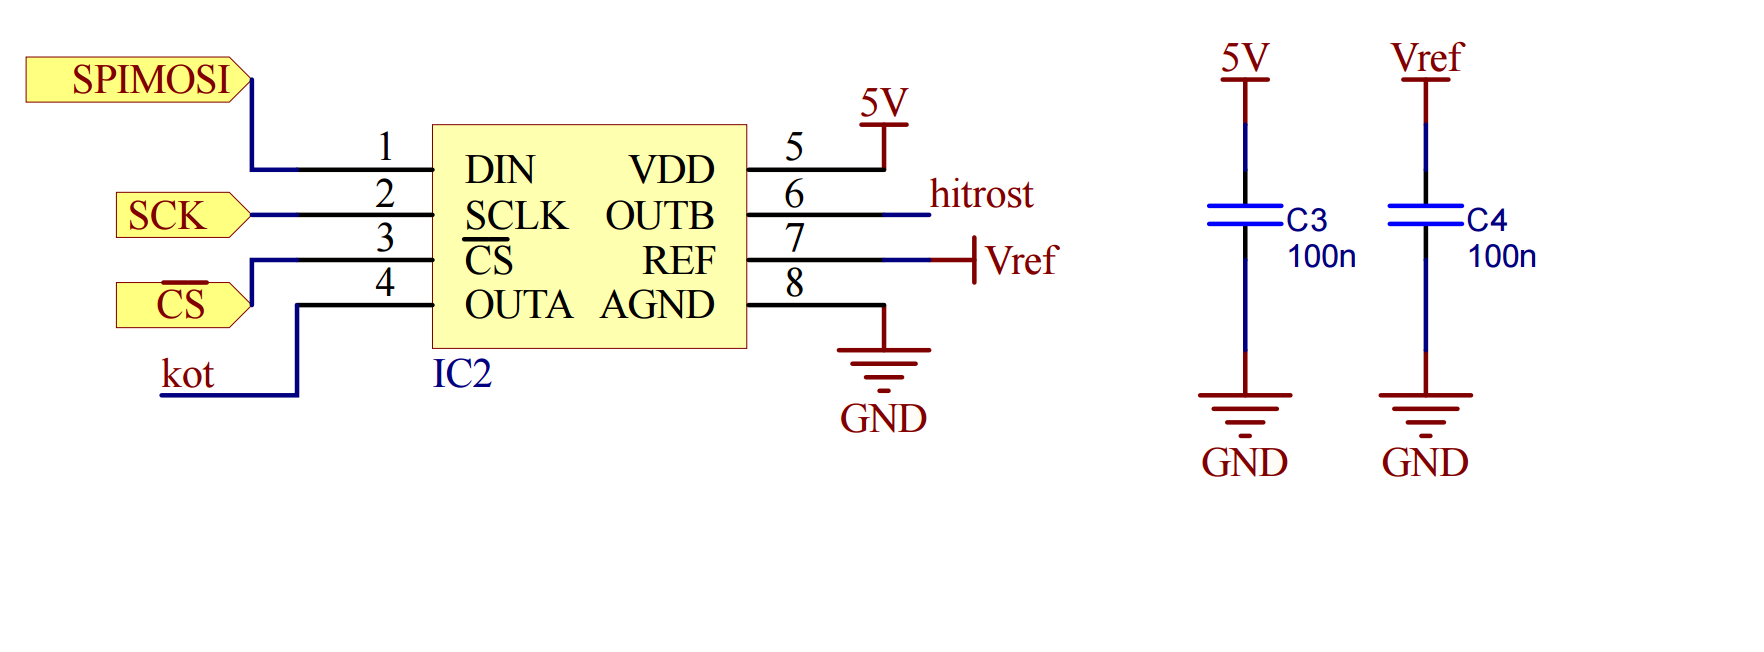
\includegraphics[width=0.7\textwidth]{DAC.png}
		\caption{Shema DAC-a}
		\label{DACshema}
	\end{figure}



Operacijske oja"cevalnike bi moral le prerisati, oja"cenje pa zmanj"sati za polovico. Sam sem sestavil le blok kot skupek 4 oja"cevalnikov. Ob povezovanju sem naredil napako, da sem na  oja"cevalniku C zamenjal vhoda. Tako sem naredil pozitivno povratno zanko in posledi"cno vezje ni ustrezalo od"stevalniku (Slika~\ref{OPshema}).


	\begin{figure}[!h]
		\centering
		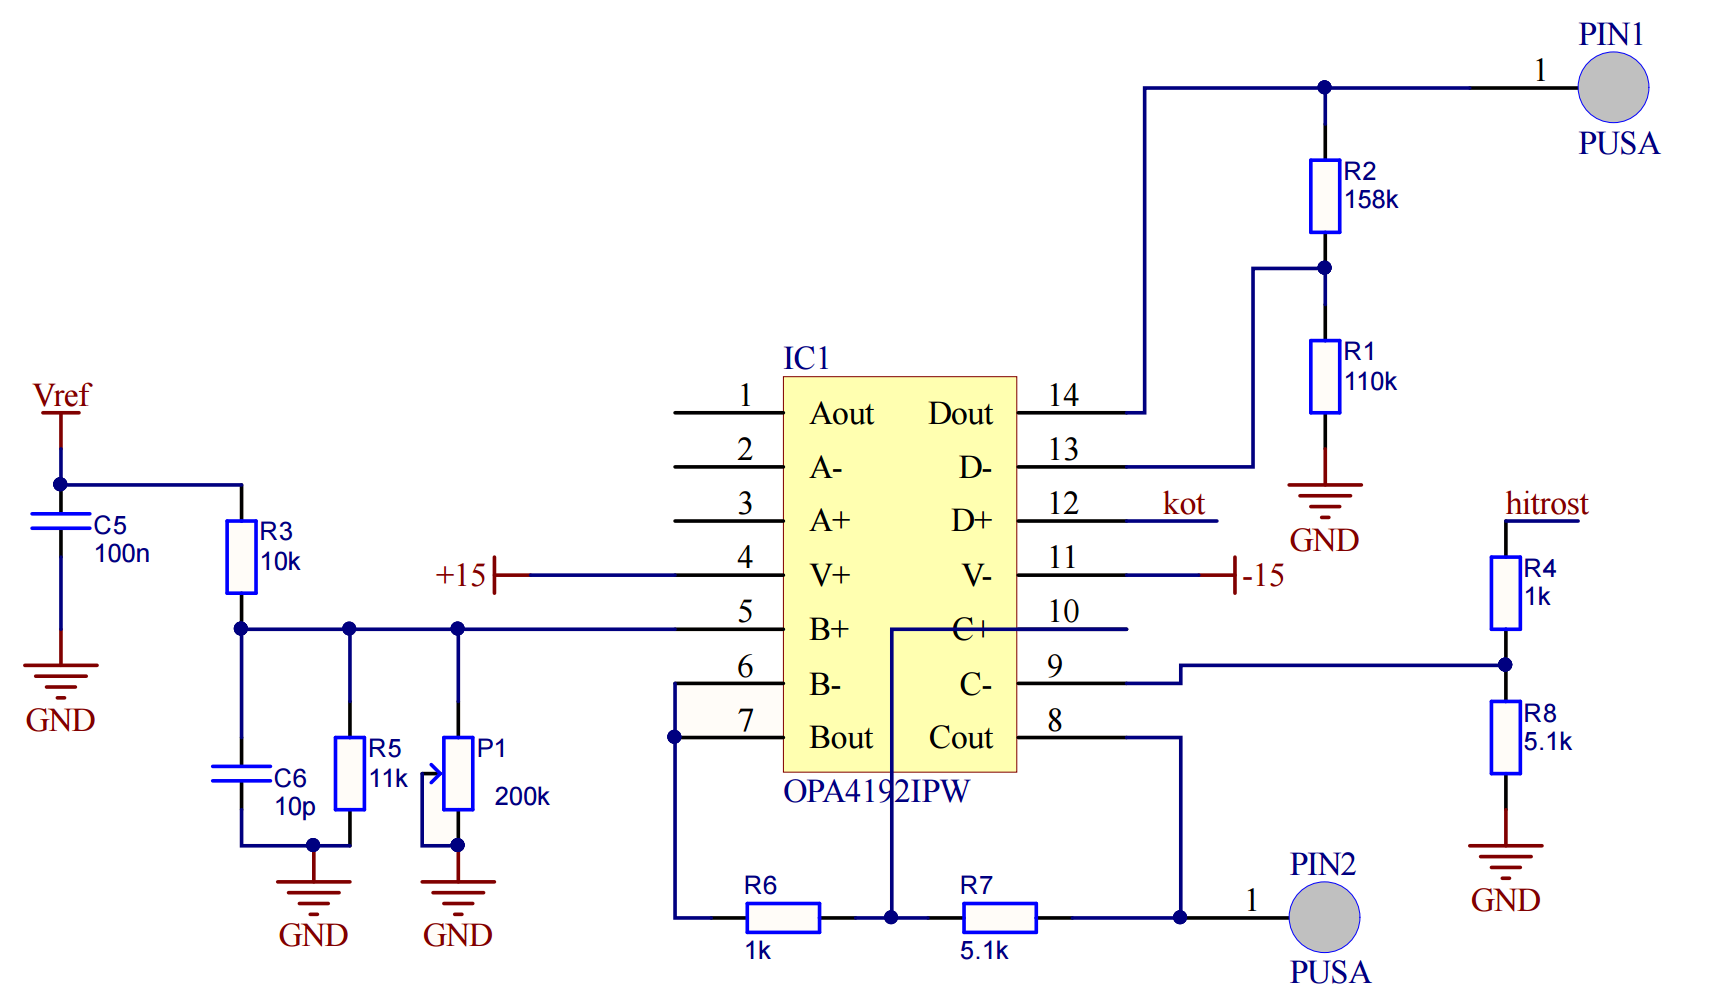
\includegraphics[width=\textwidth]{OP.png}
		\caption{Shema operacijskega oja"cevalnika}
		\label{OPshema}
	\end{figure}


\section{Izdelava tiskanine}

Ko sem shemo, po mojem mnenju zaklju"cil, sem se lotil postavitve elementov na dvoplastno tiskanino. Rezultat je na sliki \ref{PCB}.

	\begin{figure}[!h]
		\centering
		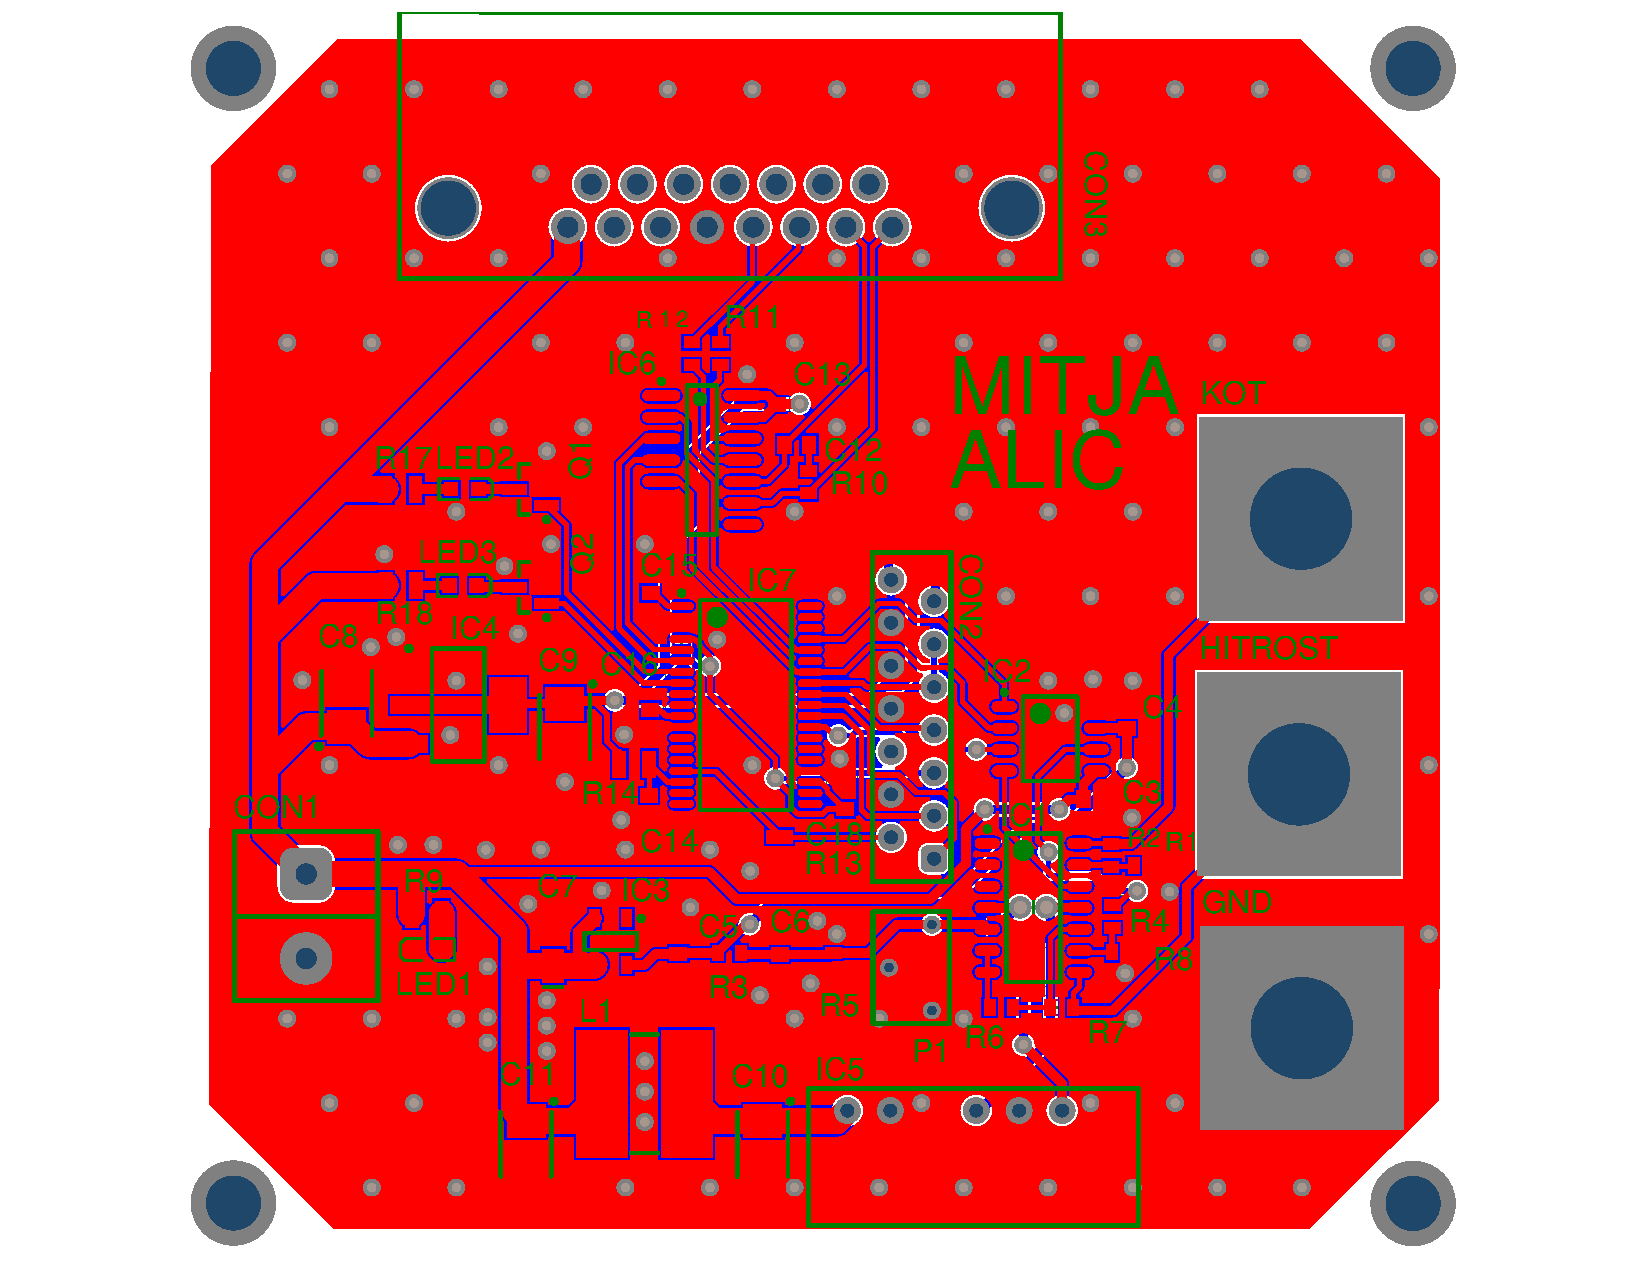
\includegraphics[ width=\textwidth]{Merilnik_2017_01_13.pdf}
		\caption{Izgled tiskanine katera je "sla v izdelavo}
		\label{PCB}
	\end{figure}

 
 "Footprint-e"~sem nastavil "ze na shemi, zato se s tem tu nisem ukvarjal. Vse napake na tiskanini, so posledica nenatan"cnosti pri na"crtovanju sheme. Konektor za napajanje sem izbral tako, da je bilo potrebno vanj vija"citi napajalni "zici. Naslednik naj uporabi konektor, katerega lahko izklopi brez kak"snih potrebnih pripomo"ckov. Sam sem postavil na tiskanino upore in kondenzatorje velikosti 0603\footnote{Imperialne enote, v metri"cnem sistemu je to 1608}. V laboratoriju LRTME ponavadi uporabljajo komponente velikosti 0805, zato jih je bilo potrebno na Farnell-u naro"citi. Najprej sem s pomo"cjo Aleksandra Abramovi"ca naspajkal mikrokrmilnik, nato pa nadeljeval z upori ter kondenzatorji okoli mikrokrmilnika. Naspajkal sem vse razen napajalnika za napetost $\mathrm{\pm}$15V in DAC-a. DAC-a ob naro"canju materiala na Farnell-u ni bilo ve"c na zalogi, zato sem ga naro"cil na Mouser-ju. Ko sem prvi"c priklopil vezje na napetostni vir, sem napajalno napetost po"casi vi"sal in opazoval vhodni tok. "Se preden sem za"cel vezje programirati sem prevezal pina na oja"cevalniku C, katera sem v shemi zamenjal. Preko Texas Instruments XDS100v2 USB Debug Probe sem priklopil vezje na ra"cunalnik in lahko za"cel programirati v Code Composer Studio.

\section{Programiranje}
Programirati sem za"cel v koncu februarja 2017.
Projekt z za"cetnimi header datotekami, osnovnimi inicializacijami mikrokrmilnika in prekinitvijo mi je pripravil mentor. Potek programirannja sem si zadal po naslednjem seznamu:
\begin{itemize}
\item Za"zeni PWM enoto za krmiljenje LED diod
\item Uredi komunikacijo s senzorjem zasuka
\item Dodaj algoritem alfa beta filtra za izra"cun hitrosti
\item Uredi komunikacijo z DAC-om
\end{itemize}

\subsection{PWM enota}

Za PWM enoti sem moral pina GPIO~4 in GPIO~5 nastaviti za PWM izhoda. Nastavil sem registre tretjega modula PWM, kateremu pripadata izhodna pina. Ob \mbox{reset-u} programa sta prikazovalni LED diodi prikazovali naklju"cna stanja saj se je izhod PWM enote postavil v visoko impedan"cno stanje, pull-down upora na gate-u tranzistorja pa ni bilo.

\subsection{Povezava s senzorjem zasuka}

Pri predmetu DP2 sem dobil "ze napisano inicializacijo in zajem kota po SPI komunikaciji. Potrebni datoteki (SPI\_ dajalnik.h in \mbox{SPI\_ dajalnik.c}) sem dodal v projekt. Nastaviti sem moral "se pina za krmiljenje "cipa za spremembo komunikacije (DE na GPIO~2 in RE na GPIO~3). Nastavil sem ju na vrednosti tako, da je bila komunikacija ves "cas mogo"ca. Ko sem "zelel preveriti delovanje se je hitro pokazalo nedelovanje. Za vrnjen podatek sem dobil le invertiran urin signal. To je bila posledica mo"skega "\mbox{footprint-a}"~konektorja za povezavo s senzorjem. Zaradi zrcaljne slike je bila "zica katera napaja senzor vezana na pin CLK+. Senzor se je s tem signalom le pri"zigal in uga"sal. To napako sem re"sil tako, da sem konektor odstranil z zgornje strani tiskanine in ga prispajkal na spodnjo stran. S tem posegom sem izhodne pine konektorja spravil na pravo mesto in komunikacija je delovala.

\subsection{Algoritem za izra"cun hitrosti}  

Kodo za izra"cun vrtilne hitrosti sem napisal "ze pri vajah predmeta DP2. Vrnjen rezultat je bila frekvenca in ne vrtilna hitrost, ki je le za faktor 2$\mathrm{\pi}$ skalirana. V programu sem ra"cunal s plavajo"co vejico (na procesorju TMS320f28069). Ko sem dodal to kodo v moj mikrokrmilnik, se  kode ni uspela izvajati dovolj hitro. Alogritem sem zato pretvoril na ra"cunaje s fiksno vejico\footnote{Uporabil sem format f8.24}. Algoritem se nahaja v \nameref{Dodatek2}. Uporabil sem knji"znico IQ\_ math. Algoritem  se tako izvede v dovolj kratkem "casu, "casa pa nisem pomeril.


\subsection{Povezava z digitalno analognim pretvornikom}

Ko sem dobil DAC in je bil algoritem za  izra"cun hitrosti dokon"can, sem naspajkal pretvornik na tiskanino. Ob priklju"citvi na napetostni vir, tiskanina ni izkazovala nobene napake. Zato sem se lotil nastavljanja izhodov za postavitev komunikacije. Za vzpostavitev komunikacije (chip enable), sem uporabil GPIO~34, kateri ima le to funkcijo. V "datasheet-u"~nikjer drugje ni bil ni"c opisan. Vsi ostali pini imajo ve"c funkcij, zato je bil vsak pin podrobneje opisan, GPIO~34 pa ima le to funkcijo in ne potrebuje drugega opisa. Ko bi moral postaviti GPIO~34 na 0~V je imel ta konstntno 5~V. Naj omenim, da je mikrokrmilnik napajan s 3,3~V in v razponu, od 0~V do napajalne napetosti, je lahko izhod. To se mi tu "se ni posvetilo. Dvomil sem v pin GPIO~34 kateri ni bil podrobneje opisan v "datasheet-u". Zato sem na mikrokrmilniku prevezal tako, da sem chip enable pin DAC-a povezal z GPIO~19. Ta pin ima "ze funkicjijo, da se postavi v "zelejeno stanje ob za"cetku SPI komuniciranja. Vendar ta prevezava ni pomagala. Mentor je nato ugotovil napako, ki je bila ustvarjena v shemi, da so pini DAC-a na levi strani zamenjani. Na tej to"cki je mentor predlagal, da s projektom kon"cam in bo zapisan kot neuspe"sno izdelan. Nato sva ugotovila, da se lahko DAC "se preve"ze v delujo"ce stanje. 

Prevezal sem DAC in za"celo je delovati. Po tem je bilo potrebno samo "se skalirati in nastaviti vrednosti, da bo kon"cni izhod napetosti hitrosti in kota med $\mathrm{\pm}$~10V. Pojavila se je te"zava, da je izhod B DAC-a upadel za pribli"zno 1~V ko je potekala komunikacija. Tega nisem znal re"siti, slutim pa, da je bila napaka povzro"cena z dodatnimi prevezavami na tiskanini.


	\begin{figure}[!h]
		\centering
		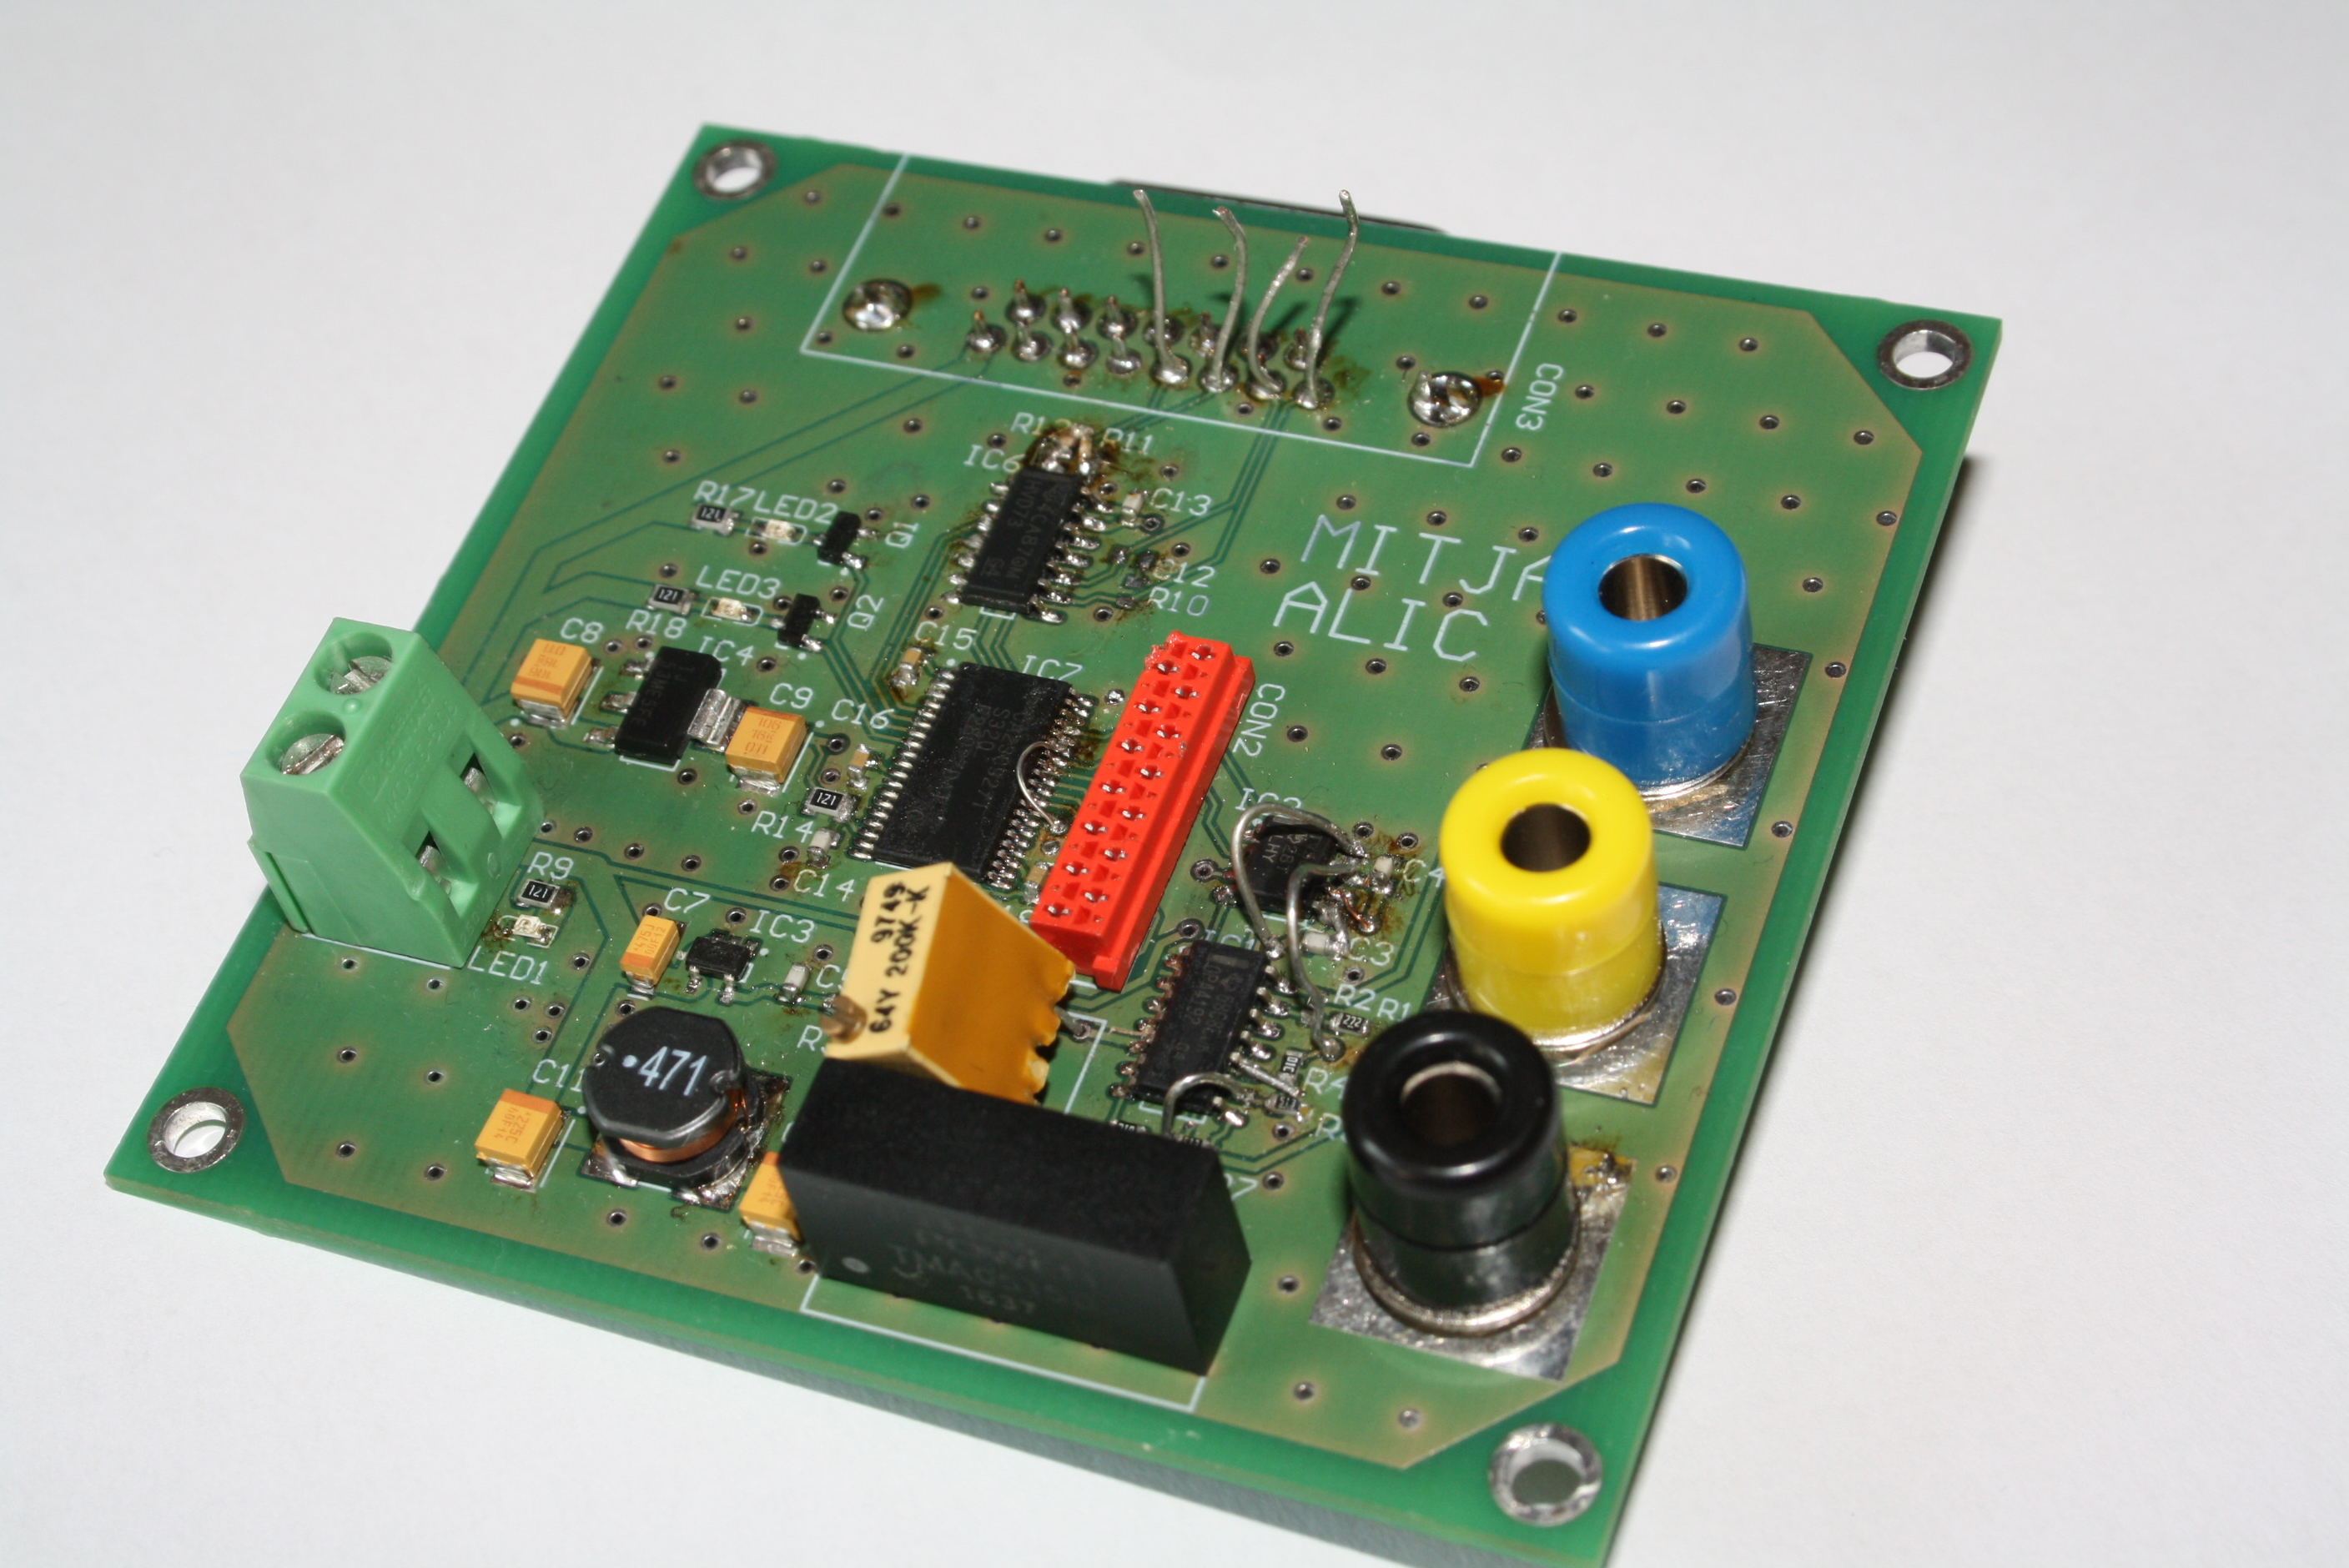
\includegraphics[ width=\textwidth]{IMG_8482.JPG}
		\caption{Tiskanina na koncu projekta}
		\label{vezje1}
	\end{figure}

\subsection{Ostale te"zave}
Nepravilno se je za"cel obna"sati tudi komunikacija s senzorjem zasuka. Kljub temu, da je senzor prejemal urin signal, ni vra"cal podatka. Podatek je vrnil "ce sem ob pravem trenutku spremenil vednost DE pina na komunikaciji iz 0 na 1. To sem ugotovil, ko sem ponesre"ci povezal pin DE s pinom SPICLK. Vrednost na pinu DE je tako prekapljala med 0 in 1 in komunikacija je nato za"cela delovati. To sem posku"sal nato dose"ci tudi s programom, tako da je preklapljal vrednost na pinu DE vendar se ni odzval vedno.

Po tednu iskanja re"sitve za nastale te"zave sem se odlo"cil in mentorju sporo"cil, da bi projekt raje zaklju"cil saj traja "ze predolgo. Projekt ni bil tako kompleksen, vendar sem si ga z napakami zakompliciral sam.

\section{Pisanje poro"cila}

V poro"cilu sem morala zbrati vse napake, ki sem jih naredil pri projektu. Hotel sem posneti oscilograme vendar sem  ob tem skuril mikrokrmilnik. Zato oscilogramov v tem poro"cilu ne boste opazili.





\section{Napake projekta}
	\subsection{Mo"ski "footprint"~za "zenski konektor}
	
	Mentor me je velikokrat opozoril ali sem resni"cno uporabil pravi "footprint"~za konektor, vendar tega ob sestavljanju sheme nisem nikoli preveril. Napaka se je pokazala ob vzpostavljanju komunikacije s senzorjem. Napako sem re"sil tako, da sem konektor prispajkal s spodnje strani tiskanine( slika \ref{vezje2}).
	\begin{figure}[!h]
		\centering
		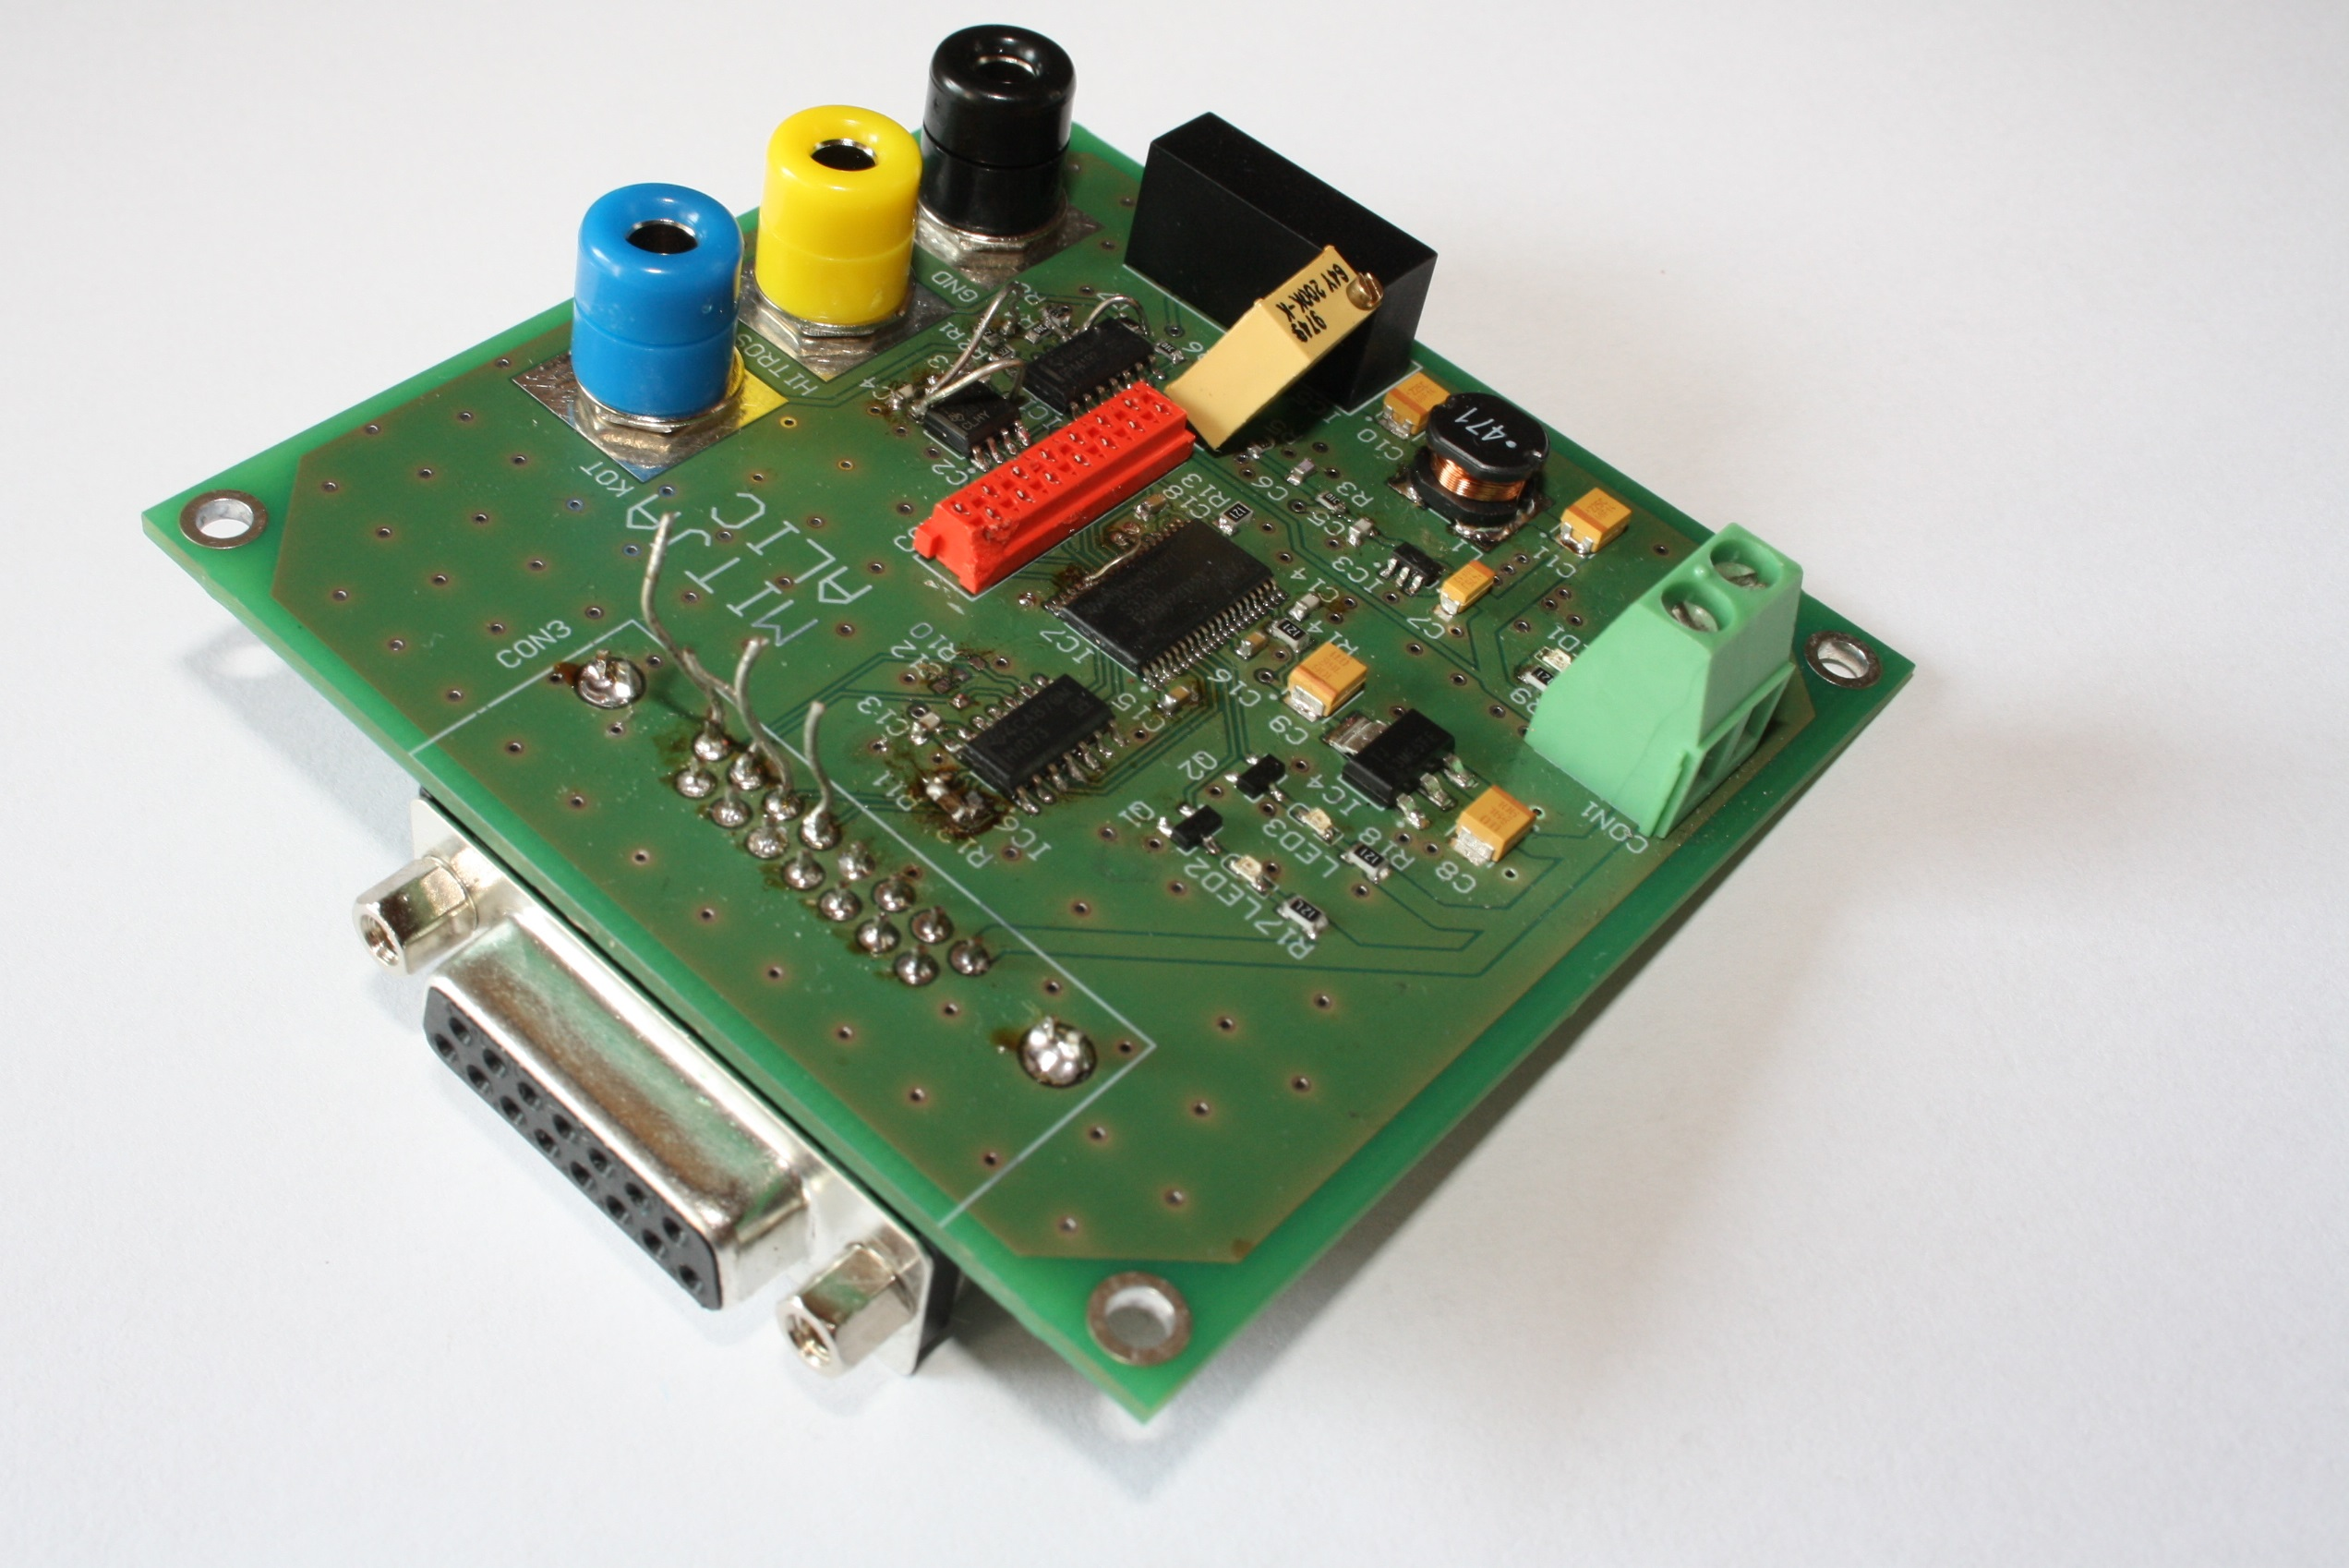
\includegraphics[ width=\textwidth]{IMG_8463.JPG}
		\caption{Konektor prispajkan na spodnji strani tiskanine zaradi anpake v "footprintu"}
		\label{vezje2}
	\end{figure}
	
	
\subsection{Priklju"cek za napajanje}

Ta napaka niti ni tako huda, je pa priporo"cljivo da se uporabi konektor katerega lahko odklopi"s, brez izvija"ca. Konektor katerega sem uporabil se vidi na desni strani slike~\ref{vezje2}.

\subsection{Pull-down upori na gate-u MOS-FETa}

Pin mikrokrmilnika je bil direktno vezan na gate tranzistorja. Ob priklju"citvi napajalne napetosti so izhodi mikrokrmilnika v visoko impedan"cnem stanju. Tranzistor je v tem stanju lahko prevajal, lahko ne. To bi re"sil upor vezan na maso in tako definiral stanje v primeru visoko impedan"cnega stanja pina na mikrokrmilniku. Prajndl je upore uporabil, jaz sem jih spustil. 


\subsection{Napaka v povezavi senzorja z vezjem}

V poglavju \ref{shema}, sem "ze opisal zamenjavo impedanc med paroma ure (CLK) in podatka (DAT). To napako sem na"sel na koncu, ko mi komunikacija s senzorjem ni delovala in sem se posvetil branju "\mbox{datasheet-a}"~senzorja RM44SI. Opazil sem, da je potrebno pri izhodnih signalih senzorja vezati 120$\mathrm{\Omega}$ upor in kondenzator, kar sem popravil. "Se ena napaka, ki me je nau"cila naj dobro berem vse podatkovne listine.


\subsection{Postavitev potenciometra poleg JTAG konektorja}

Na sliki~\ref{vezje1}, prav tako na sliki~\ref{vezje2} se vidi da potenciometer ni lepo prispajkan. Razlog je v tem, ker sem ga na tiskanini postavil preblizu konektorja JTAG. Ko sem "zelel povezati tiskanino z ra"cunalnikom, ni bilo prostora za nasaditev priklju"cka. Potenciometer sem moral tako zamakniti, da sem lahko uporabil konektor. Ob kon"cnem izdelku to niti ni napaka, saj konektor slu"zi le za povezavo z ra"cunalnikom v "casu razvijanja programa. Ja pa to "sola za naprej, da si ob konektorjih pustim dovolj prostora. Napaka pa je bila popolnoma nepotrebna, "ce bi bil dosleden.

\subsection{Zamenjana vhoda na od"stevalniku}

Napaka, ki bi jo moral hitro opazi "ze na shemi. Povezavi na vhodu oja"cevalnika C sem obrnil. S tem  sem naredil pozitivno povratno zanko. To se je dalo popraviti s prevezavo na tiskanini. 

\subsection{Narobe konfigurirani pini na DAC-u}

Na DAC-u sem levi strani pinov pripisal napa"cne "designatorje". Na levi strani sem jih o"stevil"cil od zgoraj navzol. Na "footprint-u" pa o"stevil"cenje pinov na levi strani,  poteka od spodaj navzgor. To napako bi lahko popravil "ce bi spremenil oznake "designatorjev", ali "se la"zje v nastavitvah Pin~Map bi lahko posameznemu pinu na shemi priredil pin na "footprint-u".

\subsection{Napa"cna vrednost referen"cne napetosti}

Ob koncu projekta sem ugotovil, da moja referen"cna napetost (4,096~V), ni bila najprimernej"sa. V "\mbox{datasheet-u}" DAC-a sem opazil kasneje, da je najprimerneje uporabiti vrednost referen"cne napetosti 2,048V. Najvi"sja refern"cna napetost pa naj nebi bila vi"sja od $\mathrm{V_{DD}}$~-1,5~V. Ni klju"cna napaka je pa prav, da jo omenim.
	
	
\section{Zaklju"cek}


	V projektu sem ustvaril lepo zbirko napak. Ve"c ali manj jih je bilo proizvedenih med izdelavo sheme, katere sem se lotil zelo lahkotno. Ta lahkotna misel pri sestavi sheme, me je pripeljala do neuspe"snega zaklju"cka. S tem projektom sem se po mojem mnenju na nekoliko bole"c na"cin npridobil dosti ve"c novega znanja in bom zato v prihodnosti bolj dosleden. 
\newpage

\pagestyle{empty}
	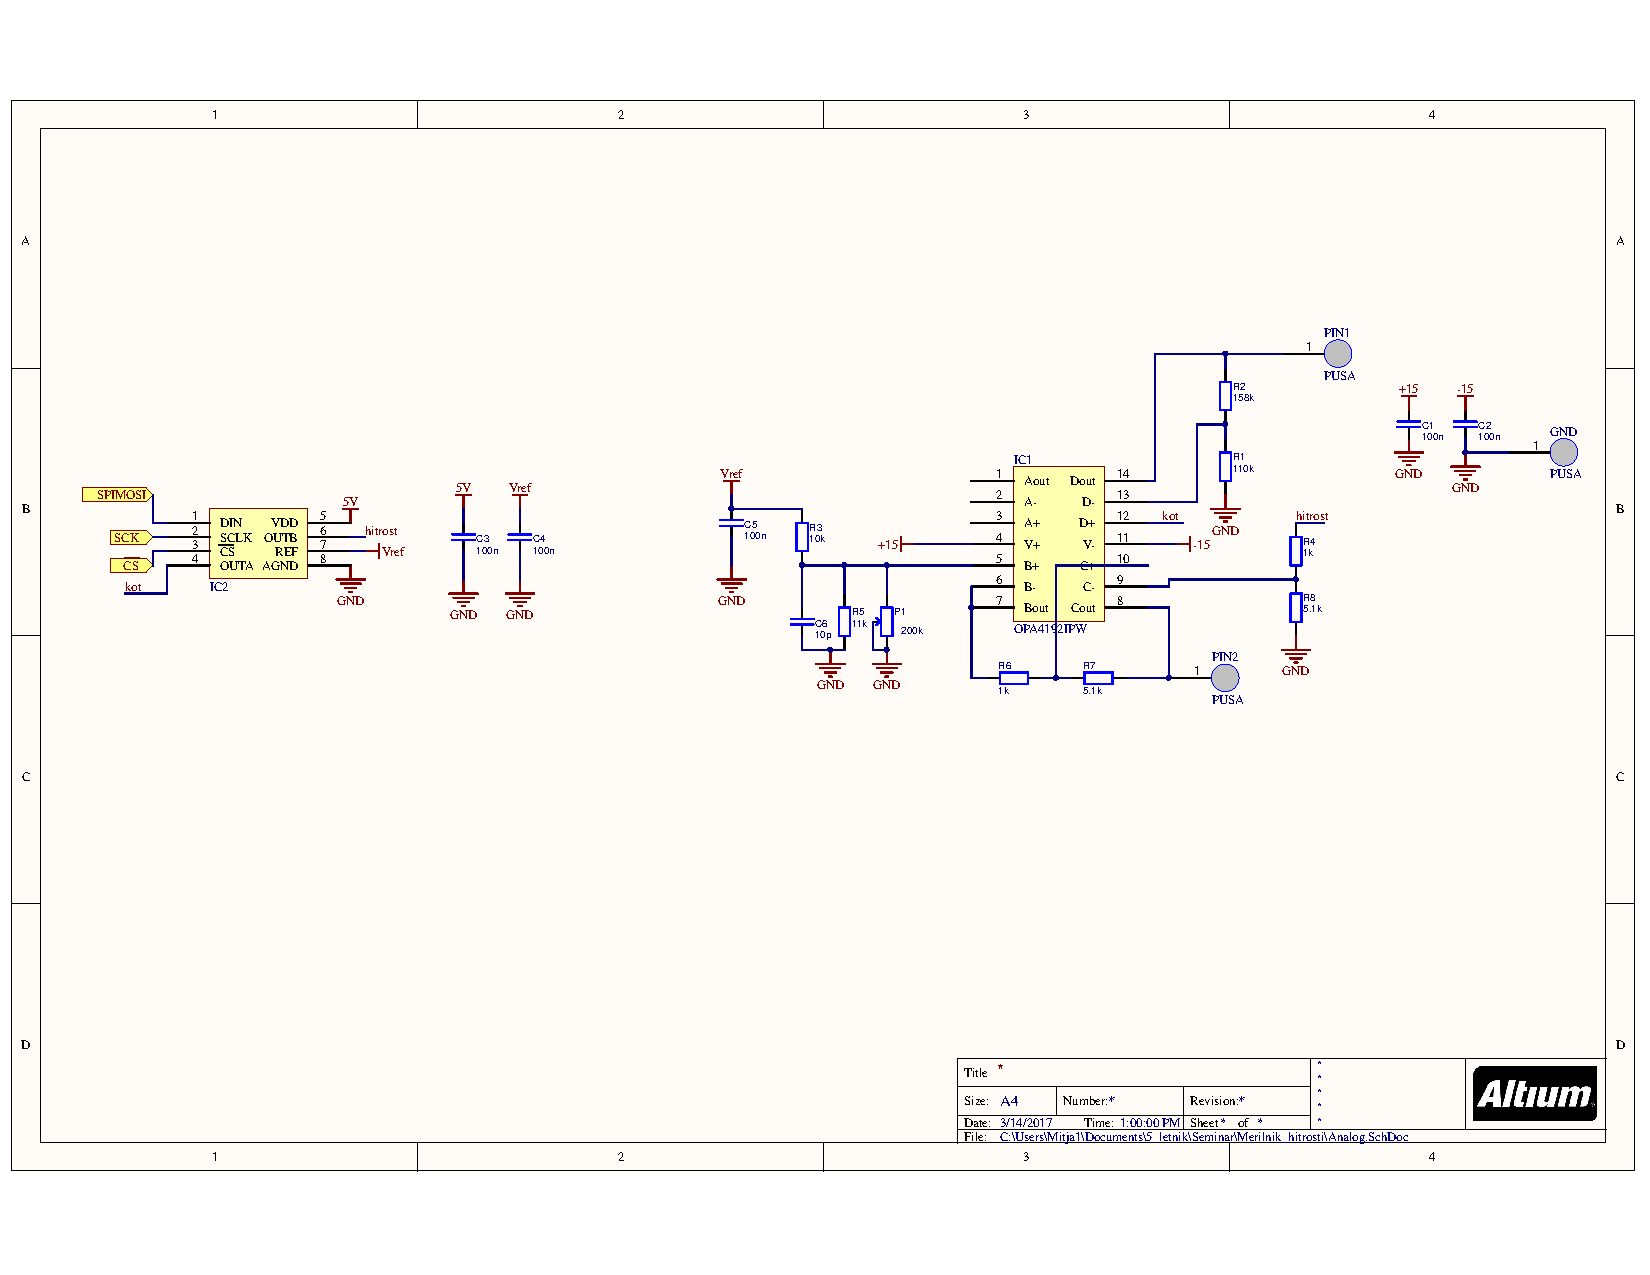
\includepdf[pagecommand=\section{Dodatek 1}\label{Dodatek1}, page=2,angle=-90]{Merilnik_hitrosti.pdf}
	
	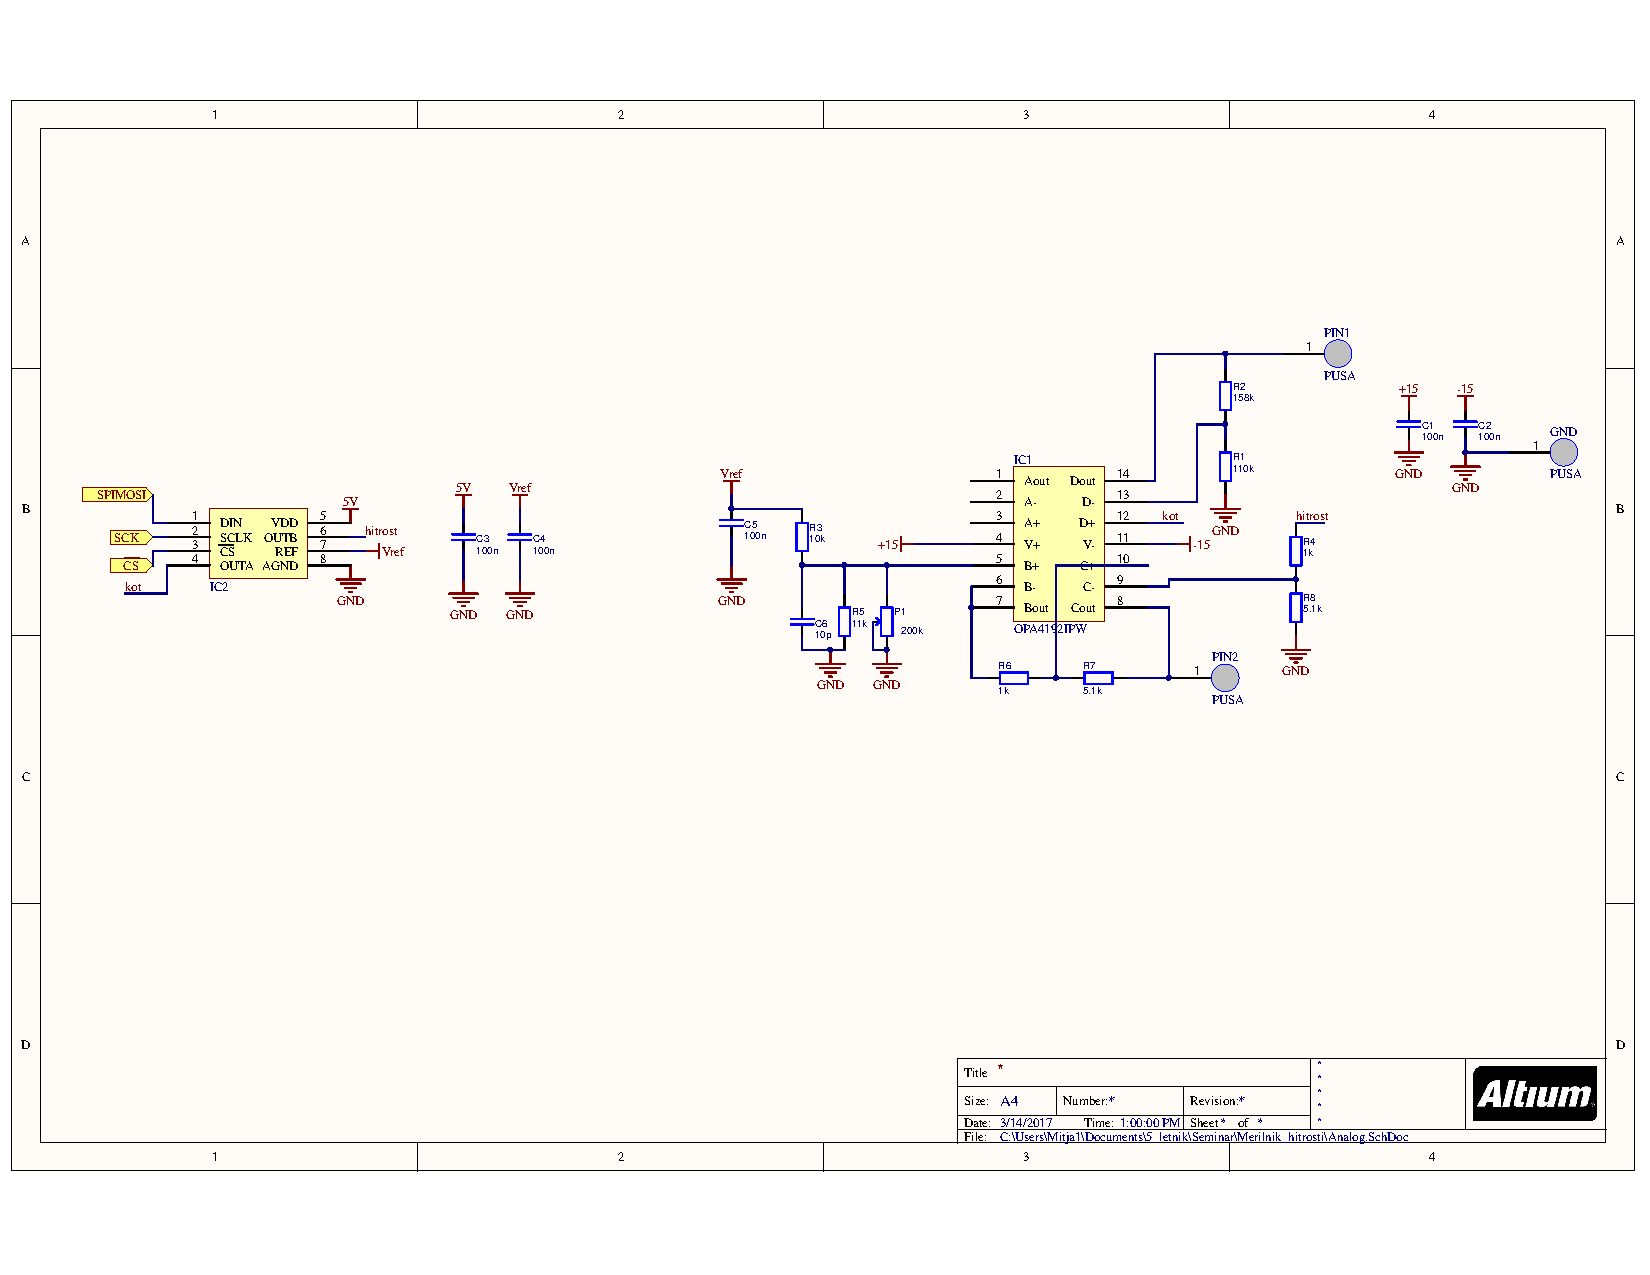
\includepdf[ page=3,angle=-90]{Merilnik_hitrosti.pdf}
	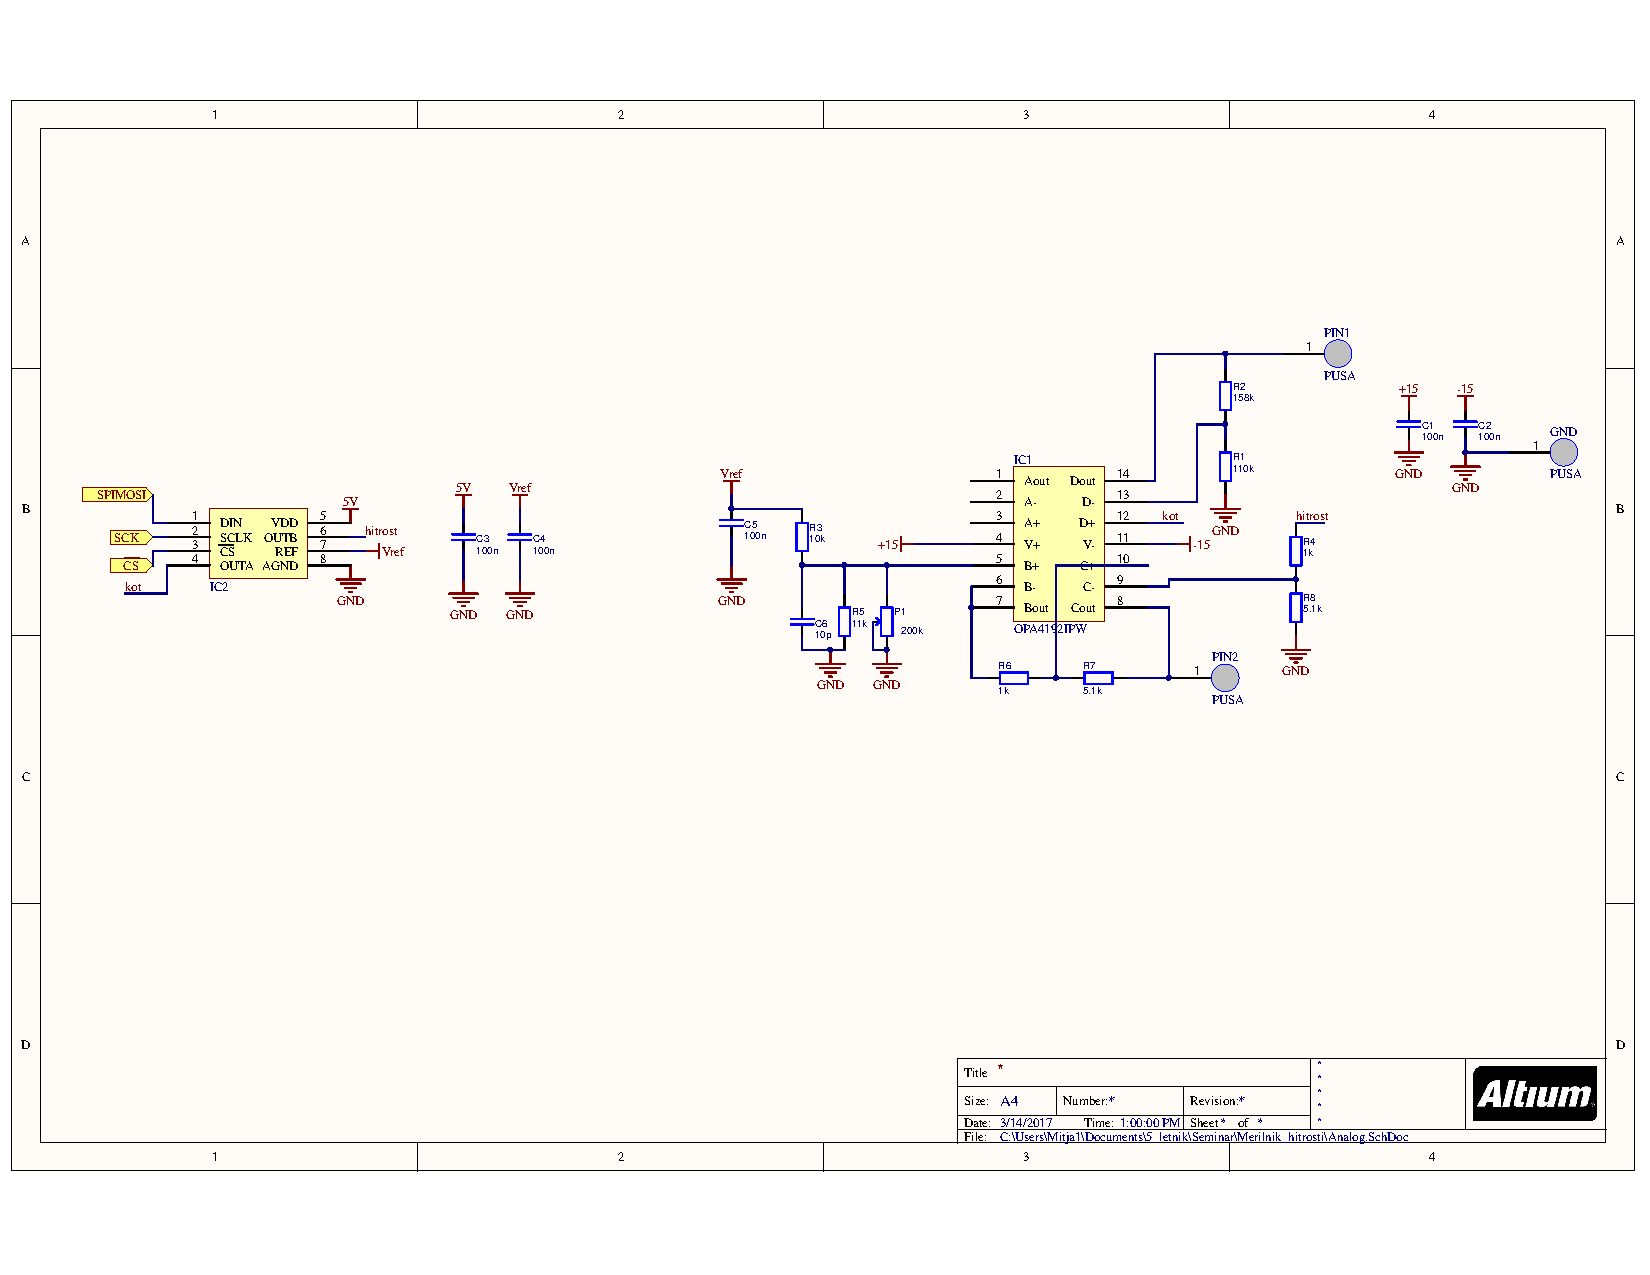
\includepdf[ page=1,angle=-90]{Merilnik_hitrosti.pdf}
\newpage
\pagestyle{fancy}
\section{Dodatek 2}
\label{Dodatek2}
Algoritem alfa beta filtra sem sestavil po predlogi iz magistrskega dela Repetitivna regulacija hitrosti sinhronskega stroja s trajnimi magneti, Denisa Su"sina, Univerza v Ljubljani, 2016 stran 39,40.
\begin{verbatim}

	kot_abf+=_IQmpy(f_abf,dt); //kot_abf je spremenljivka ki ima vrednost 
	                           //ze iz prejsnje prekinitve
	if(kot_abf>_IQ(1.0))	// kot_abf je v p.u. zato se nahaja med 0.0 in 1.0
		{
			  kot_abf-=_IQ(1.0);
		}
	if(kot_abf < 0 )
		{
			  kot_abf +=_IQ(1.0);
		}
		
	epsilon= (kot_iz_senzorja<<12)- kot_abf; //kot_iz_senzorja je 12 biten 
	                                         //pretvorim v f8.24 p.u.
	if(epsilon >= _IQ(0.5)) // odprava prehoda iz 0.9999 na 0
		{
			  epsilon-=_IQ(1.0);
		}
	if(epsilon <= _IQ(-0.5) )
		{
			  epsilon +=_IQ(1.0);
		}
		
	kot_abf+=_IQmpy(alpha,epsilon); //definicija popravlejnega kot_abf 
	                                //za naslednjo prekinitev

	f_abf+=_IQmpy(epsilon,_IQdiv(betha,dt)); //definicija popravlejnega 
	                                         // f_abf za naslednjo prekinitev
\end{verbatim}


\end{document}
